\subsection{Language Details}
\subsubsection{Data Types}
There is only one data type in BLAStoff, the matrix.  Matrices can be defined four ways: as a matrix literal, as a graph, as a number, or with a generator function.
\paragraph{Matrix Literal Definition}
A matrix literal looks as follows:
\begin{lstlisting}
M = [1,3,5;
     2,4,6;
     0,0,-1];
\end{lstlisting}
which sets M as the matrix $$\begin{bmatrix}1&3&5\\2&4&6\\0&0&-1\end{bmatrix}$$.
The values given to $M$ can be anything $\in \mathbb{R}\cup \pm\infty$.  Here's an example of using values that aren't just integers:
\begin{lstlisting}
M = [1.2, inf;
    -inf, -34];
\end{lstlisting}
which sets M as the matrix $$\begin{bmatrix}1.2&\infty \\ -\infty & -34\end{bmatrix}$$.
\paragraph{Graph}
The graph definition looks as follows:
\begin{lstlisting}
G = {
    0->1;
    1->0;
    1->2;
    4;
};
\end{lstlisting}
This will set $M$ as the adjacency matrix for the graph described, which in this case would be: $$\begin{bmatrix}0&1&0&0&0\\1&0&1&0&0\\0&0&0&0&0\\0&0&0&0&0\\0&0&0&0&0\end{bmatrix}$$  As we can see in this code example, each line in the graph definition can be an edge $a\to b;$ defining a node between vertices $a$ and $b$ where $a,b$ are non-negative integers, or just a vertex $c;$ where $c$ is also a non-negative integer, which just defines that the vertex $c$ exists.  The matrix created will be an $n \times n$ matrix, where $n$ is the highest vertex (in our case 4) defined plus 1.  Thus, the graph created will have nodes $[0,n-1]$.  Any vertices not mentioned in the definition but in the range $[0,n-1]$ will be created, but not have any edges to or from it (such as vertex 3 in this case).  We could easily extend this syntax to allow for bi-directional or weighted graphs, and will decide later whether to do this.

\paragraph{Number Definition}
The number definition is quite simple, and looks like as follows:

\begin{lstlisting}
M = 5;
\end{lstlisting}
This is how you would create a  ``scalar'' in BLAStoff, but because the only data type is a matrix, scalars are really $1\times 1$ matrices.  The above code is equivalent to the following code:
\begin{lstlisting}
M = [5];
\end{lstlisting}
which sets $M$ as the matrix $$\begin{bmatrix}5\end{bmatrix}$$
A potential issue could be that not allowing scalars means you can't have scalar multiplication, but we define a convolution operator, which ends up working like scalar multiplication if the right hand side is a $1\times 1$ matrix.

\paragraph{Generator Function Definition}
We also have a number of generator functions for commonly-used types of matrices so that you don't waste your time typing out a $50 \times 50$ identity matrix.  The first is the \verb=Zero= function, which generates a matrix with all 0s.  This takes in one argument, which we will call $x$, a non-negative integer matrix of two possible sizes.  $n$ can be a $2 \times 1$  positive  integer matrix, and the elements of the $n$ matrix are the height and width of the zero matrix, in that order.  $n$ could also be a $1\times 1$ matrix, in which case the zero matrix will be square, with the element in $n$ as its height and width.  Here is an example:

\begin{lstlisting}
A = Zero(4);
B = Zero([3;2]);
\end{lstlisting}
This code would result in the following matrices:
$$A=\begin{bmatrix}0&0&0&0\\0&0&0&0\\0&0&0&0\\0&0&0&0\end{bmatrix}$$
$$B=\begin{bmatrix}0&0\\0&0\\0&0\end{bmatrix}$$
Note that \verb|A = Zero(4);| is equivalent to \verb|A = Zero([4;4]);|.

We also have an identity function, \verb=I=, which takes in one argument, a $1\times 1$ non-negative integer matrix, the width and height of the resultant square identity matrix.  Example:\begin{lstlisting}
M = I(3);
\end{lstlisting}
This would result in the following matrix:
$$M=\begin{bmatrix}1&0&0\\0&1&0\\0&0&1\end{bmatrix}$$
The final generator function is the \verb=range= function, which generates a column vector that goes through an integer range, incremented by 1.  Like \verb=Zero=, it takes in an integer matrix of size $1\times 1$ or size $2\times 1$, which gives the bounds of the range generated (inclusive lower, exclusive upper), or, in the $1\times 1$ case, the exclusive upper bound, and 0 is the default lower bound.  Here are some examples:
\begin{lstlisting}
A = range(3);
B = range(-2,2);
\end{lstlisting}
This code would result in the following matrices:
$$A = \begin{bmatrix}0\\1\\2\\3\end{bmatrix}$$
$$B = \begin{bmatrix}-2\\-1 \\0\\1\\2\end{bmatrix}$$
If a range where the lower bound is greater than the upper bound given to \verb=range=, such as \verb=range([5;-1])=, a $0 \times 1$ matrix will be returned.

\paragraph{Integers vs. Floats}
You're probably confused now, because I said earlier that the only type in BLAStoff is a matrix, but now I'm talking about integers and floats?  So, while in a perfect world we could just have everything be floats, as we're defining our linear algebra over the reals, consider the following code if (which makes use of a few operators we will define below, but you can guess how it generally works for now):
\begin{lstlisting}
b = 25020359023950923059124;
a = 2;
M = [1,2;3,4];
a += b;
a -= b;
M = M^a;
\end{lstlisting}
If this code has no floating point errors, than the final line is just a simple matrix squaring.  However, if some error is introduced to \verb=a=, then we have a problem where we're trying to calculate something like $M^{2.000001}$, which is a much more difficult problem even if it would result in a numerically similar result.  So, I was lying a little.  Though you don't declare any types explicitly, each matrix is implicitly a float matrix or an integer matrix depending on if it is defined with any non-integers (you can only get float matrices with the literal definition).  Any operation (such as matrix addition or matrix multiplication) between a float matrix and an integer matrix results in a float matrix, while an operation between two matrices of the same type will result in a matrix of the same type, except for something like matrix inversion.


\subsubsection{Comments}
Comments in BLAStoff use C style, with \verb=//= for a single line and \verb=/*= and \verb=*/= for multi-line comments.  For example:
\begin{lstlisting}
A = 6; // I'm a comment!
B = 5; /* I'm a comment also but
...
...
I'm longer!*/
\end{lstlisting}

\subsubsection{Functions}
Functions in BLAStoff are defined with a mix of Python and C style:
\begin{lstlisting}
def foo(A, B) {
    return A;
}
\end{lstlisting}
Because there is only one data type in BLAStoff, there is no need for argument types or return types, everything is always a matrix!  Even ``void'' functions return matrices.  Consider these two functions:

\begin{lstlisting}
def bar1(A) {
    return;
}

def bar2(A) {
    ;
}
\end{lstlisting}
These two functions both return the equivalent of Python's ``None'' in BLAStoff, a $0\times 0$ matrix.

\subsubsection{If statements}
For and while loops also look similar to C.  For example:
\begin{lstlisting}
if (A > 2) {
    A = 7;
} else if (A < -3) {
    A = 5;
} else {
    A = 0;
}
\end{lstlisting}

\subsubsection{For/While Loops}
For and while loops also look similar to C.  For example:

\begin{lstlisting}
B = 0;
for (A = [0]; A < 5 ; A+=1) {
    B+=1;
}

while (B > -1) {
    B-=1;
}
\end{lstlisting}
We allow for loops, but they are not usually the ideal paradigm.  The selection operator should hopefully replace much of the use for loops.

\subsubsection{Operations}
Operations are where BLAStoff gets more interesting.

We aim to implement a large subset of the basic primitives described in \cite{Gilbert} (several of which can be combined) as well as a few essential semirings.\\\\
\label{sec:semirings}
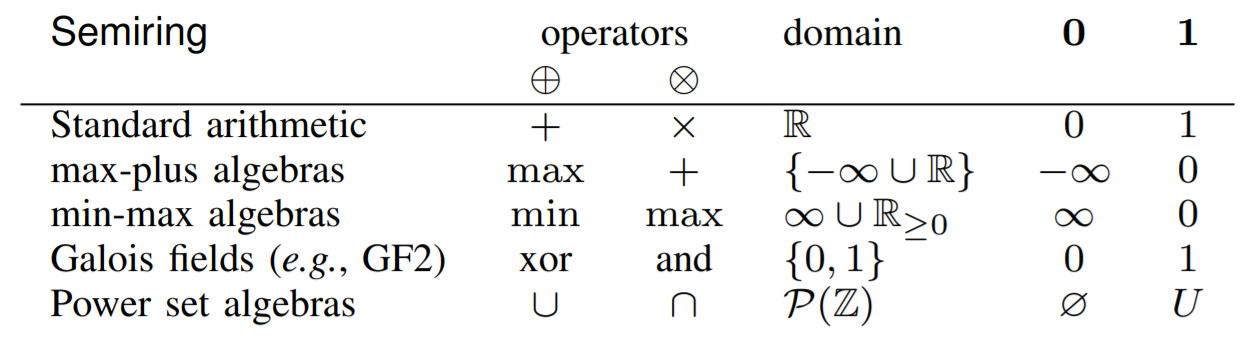
\includegraphics[scale=0.3]{figures/common Semirings.png}\\
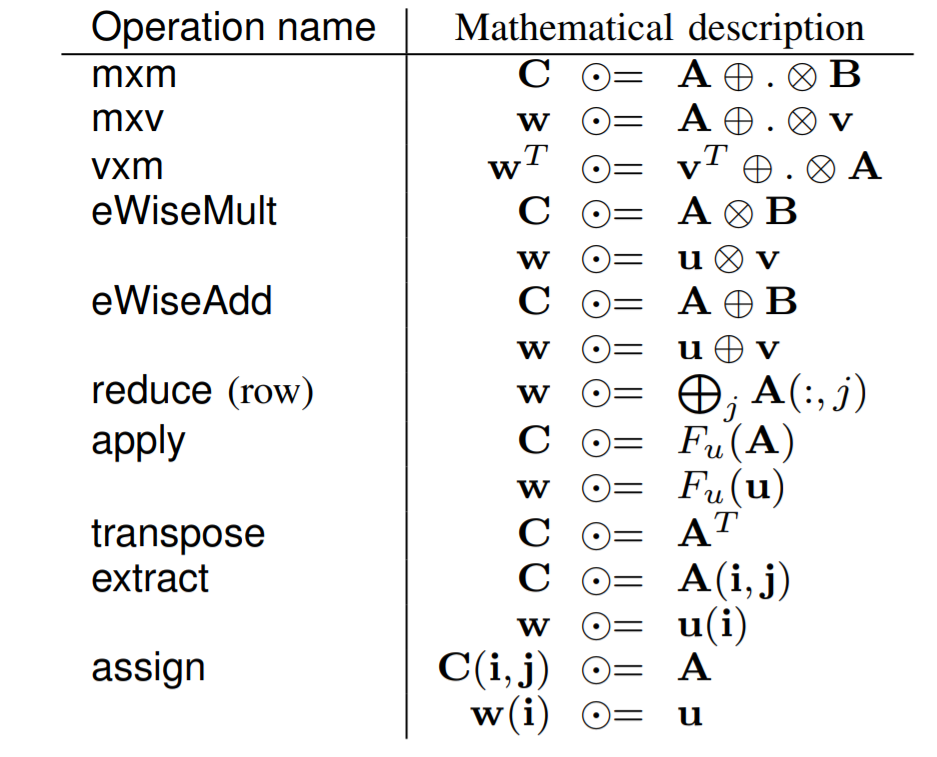
\includegraphics[scale=0.3]{figures/BLAS primitives.png}\\
Here are our operations, which implement those and more:\\
\begin{center}
\begin{tabular}{|c|c|c|}
\hline
\textbf{Name} & \textbf{Usage}\\
\hline
Assigmnent & \verb|M = N|\\
\hline
Selection & \verb=M[A, B, c, d]=\\
\hline
Matrix Multiplication & \verb=M * N=\\
\hline
Convolution & \verb=M ~ N=\\
\hline
Element-wise Multiplication & \verb=M @ N=\\
\hline
Element-wise Addition & \verb=M + N=\\
\hline
Exponentiation/Inverse/Transpose &  \verb|A^b| or \verb|A^T|\\
\hline
Size & \verb=|M|=\\
\hline
Vertical Concatenation & \verb=M : N=\\
\hline
Reduce Rows & \verb=+$M= or \verb=*$M=\\
\hline
Semiring Redefinition &  \verb=<#semiringname>= or \verb=<_>=\\
\hline
Logical Negation & \verb=<#semiringname>= or \verb=<_>=\\
\hline
Comparisons & \verb|==|, \verb|!=|, \verb|>|, \verb|>=|, \verb|<|, \verb|<=|\\
\hline
Assignment Variants &  \verb|*=|, \verb|.=|, \verb|@=|, \verb|+=|, \verb|^=|, \verb|:=|\\
\hline
\end{tabular}
\end{center}
Some of these operators' behaviors are intuitive, but we will explained further the two less intuitive ones:

\paragraph{Selection []}
The BLAStoff selection operator can be applied to any matrix looks like one of the following three forms:
\begin{lstlisting}
M[A, B, c, d];
M[A, B]
M[A];
\end{lstlisting}
where $A,B$ are column vectors of non-negative integers ($n\times 1$ matrices) and $c,d$ are $1 \times 1$ non-negative integer matrices.  $c,d$ are optional and have a default value of $\begin{bmatrix}1\end{bmatrix}$. $B$ is also optional and its default value is $\begin{bmatrix}0\end{bmatrix}$.  Abstractly, the way this operator works is by taking the Cartesian product of $A,B$, $R=A\times B$, and for each $(j,i)\in R$, we select all the sub-matrices in $M$ with a top-left corner at row $j$, column $i$, height of $c$, and width of $d$.  (BLAStoff is 0-indexed.)  This Cartesian makes the select operator a very powerful operator that can do things like change a specific of indices, while also being general enough to allow for simple indexing.  Take the following code example:
\begin{lstlisting}
M = Zero(4)
M[[0;2], [0;2]] = 1;
\end{lstlisting}

This would result in the following matrix:
$$M = \begin{bmatrix}
1 & 0 & 1 & 0\\
0 & 0 & 0 & 0\\
1 & 0 & 1 & 0\\
0 & 0 & 0 & 0
\end{bmatrix}$$
as in this case $R=\{(0,0), (0,1), (1,0), (1,1)\}$, so for every $1\times 1$ matrix at each point in $R$, we set the value to 1.  Note that the matrix on the right hand side must be of size $c\times d$.  That was a relatively complicated use of the select operator, but simple uses still have very easy syntax:
\begin{lstlisting}
M = Zero(2);
M[1, 0] = 1;
N = Zero(3);
N[1, 1, 2, 2] = I(2);
\end{lstlisting}
This would result in:
$$M=\begin{bmatrix}0 & 0 \\ 1 & 0\end{bmatrix}$$
$$N=\begin{bmatrix}
0 & 0 & 0\\
0 & 1 & 0\\
0 & 0 & 1\end{bmatrix}$$
The reason why 0 is the default value of  $B$ is to allow for easy column vector access.  Example:
\begin{lstlisting}
v = [1;1;1];
v[1] = 2;
u = [1;1;1];
u[[0;2]] = 2;
\end{lstlisting}
This would result in:
$$v=\begin{bmatrix}1\\2\\1\end{bmatrix}$$
$$u=\begin{bmatrix}2\\1\\1\end{bmatrix}$$
Now, perhaps it is clear why we included the \verb=range= generator function.  Example:
\begin{lstlisting}
v = Zeroes([5;1]);
v[range(5)] = 1;
\end{lstlisting}
This would result in:
$$v=\begin{bmatrix}1\\1\\1\\1\\1\end{bmatrix}$$
As you'd expect, trying to access anything out-of-bounds with the selection operator will throw an error.

We have shown the selection operator so far as a way of setting elements in a matrix, but it's also a way of extracting values from a matrix, as we will show below:
\begin{lstlisting}
A = [1,2,3;
    4,5,6;
    7,8,9];
B = A[0, 0, 2, 2];
\end{lstlisting}
This would result in:
$$B=\begin{bmatrix}1 & 2\\4 &5 \end{bmatrix}$$
Extraction is quite understandable when $A$ and $B$ are $1\times 1$, as that results in only one matrix, but it is a bit more complicated when they are column vectors.  In that case, we concatenate the number of resultant matrices, both vertically and horizontally.  I think an example makes this clearer:
\begin{lstlisting}
A = [1,2,3;
    4,5,6;
    7,8,9];
B = A[[0;2], [0;2] , 1, 1];
v = [1;2;3;4];
u = v[[0;2;3]];
\end{lstlisting}
This would result in:
$$B=\begin{bmatrix}1 & 3\\7 &9 \end{bmatrix}$$
$$u=\begin{bmatrix}1\\3\\4\end{bmatrix}$$


\paragraph{Semiring redefinition \texorpdfstring{$<>$}{<>}}
You may have noticed that though we have defined a number of operations on matrices, we want a way to control which operations are used on the elements of these matrices beyond standard arithmetic $+$ and $\times$.  We want to be able to use a number of semiring operators, such as those defined in \hyperref[sec:semirings]{the image above}.  BLAStoff allows for semiring redefinition in one of the following forms:
\begin{lstlisting}
<#logical>
<#arithmetic>
<#maxmin>
<_>
\end{lstlisting}
So what does this syntax actually do?  Ignore the underscore case for now.  The other three are commands to switch the command to the one denoted in the brackets.  Let's see an example:

\begin{lstlisting}
a = 2.1;
b = 3;
c = 0;

<#arithmetic>;
a + b; //returns 5.1
a * b; //returns 6.3
a * c; //returns 0

<#logical>;
a + b; //returns 1: plus is now logical or; 0 is the only false value and 1 is the default true value
a * b; //returns 1 as well: times is now logical and
a * c; //returns 0


<#maxmin>;
b + c; //returns 2.1; plus is now minimum
a * b; //returns 3; times is now maximum
a * c; //returns 5.1
\end{lstlisting}
\verb=#arithmetic= is the default, so that line was technically redundant, but included for clarity.
The example we gave was with $1\times1$ matrices, but the semiring definitions work on matrices of any size:

\begin{lstlisting}
A = [1,4;
    6,3];
B = [5,2;
    7,1];
C = A+B;
\end{lstlisting}
This would result in:
$$C=\begin{bmatrix}
1&2\\
6&1
\end{bmatrix}$$
Semiring redefinition generally is reset back to the default arithmetic when you call a function:
\begin{lstlisting}
def add(x, y) {
    return x + y;
}

a = 4;
b = 3;
<#logical>;

a + b; // will return 1
add(a, b); // will return 7
\end{lstlisting}
But we provide the \verb=<_>= in order to solve this: calling that command will set the semiring to whatever it was as this function was called (or to arithmetic as a default if you're not in a function):
\begin{lstlisting}
def semiringAdd(x, y) {
    <_>;
    return x + y;
}

a = 4;
b = 3;
<#logical>;

a + b; // will return 1
semiringAdd(a, b); // will also return 1
\end{lstlisting}

\paragraph{Extensions}
We can possibly add support for max-plus or Galois, but that will be a stretch goal.  Another, possibly loftier stretch goal, is to allow custom semirings:
\begin{lstlisting}
<+, f1, i1>
<*, f2, i2>
\end{lstlisting}
where $f_1,f_2$ is the name a function defined elsewhere that has exactly 2 arguments, and $i_1, i_2$ are number literals.  This would use $f_1(a,b)$ for $a + b$ and $f_2(a,b)$ for $a \times b$.  $i_1, i_2$ are the new empty sum and product.  We will determine if this is easy/feasible/useful/reasonable.


\subsubsection{Keywords}
BLAStoff reserves the following keywords:
\begin{verbatim}
I, Zero, range, def, return, if, else, for, while, T
\end{verbatim}

\subsubsection{Memory}
BLAStoff will use pass-by-reference and copy-by-value.  Here's an example of how this will works:
\begin{lstlisting}
def f(x){
    x += 1;
}
a = 1;
f(a);
a == 1; //TRUE
a == 2; //TRUE

b = 1;
c = b;
c += 1;
c == 2; //TRUE
b == 2; //FALSE
b == 1; //TRUE
\end{lstlisting}

BLAStoff will be garbage-collected.

\subsubsection{Scope}
BLAStoff has scope shared between blocks in the same function call, but not in different function calls.   Example:
\begin{lstlisting}

a = 1;
{
    b = 2 + a; // valid
}
c = b + 1; // valid

def f(x){
    return x * (b + c); // compile-time error
}
\end{lstlisting}


\subsubsection{Libraries/Importing Functions}
There will be a way to make/use a library and import functions, but we have not settled on the syntax nor semantics.
\subsubsection{I/O}
There will be a way to use input and output, but we also have not settled on the syntax nor semantics.



\subsection{Sample Code}

\subsubsection{Some Standard Library Functions}
As we have discussed, we intend to provide a standard library that should have include a good number of the other Linear Algebra operations that aren't primitives.  Here are some examples:

\paragraph{One}
\verb=One= works exactly like \verb=Zero=, but has all 1s in the matrix:
\begin{lstlisting}
def One(size){
    A = Zero(size);
    m = size[0];
    A[range(size[0]), range(size[1])] = 1;
    return A;
}
\end{lstlisting}

\paragraph{Horizontal Concatenation}
We don't include this as an operator because it is quite easy to write as a function using vertical concatenation and transpose:
\begin{lstlisting}
def horizontalConcat(A, B){
    return (A^T:B^T)^T;
}
\end{lstlisting}

\paragraph{Plus/Times Column Reduce}
Column reduction follows similarly:
\begin{lstlisting}
def plusColumnReduce(A){
    <_>;
    return ((+$A)^T)^T;
}

def timesColumnReduce(A){
    <_>;
    return ((*$A)^T)^T;
}
\end{lstlisting}

\paragraph{Sum}
\verb=sum= gives you the sum of all the elements in the matrix.  There are two simple $O(N)$ implementations (where $N$ is the total number of elements in the matrix), and I'll provide both options as an example:
\begin{lstlisting}
def sum(A){
    <_>;
    return A~One(|A|);
}

def sum(A){
    <_>;
    return plusColumnReduce(+$A);
}
\end{lstlisting}

\paragraph{Range From Vector}
\verb=rangeFromVector= takes in a column vector and returns a vector of the indices that have non-zero.  For instance:
$$\text{rangeFromVector}(\begin{bmatrix}
0 \\ 1 \\ 1 \\ 0 \\ 1
\end{bmatrix})
=
\begin{bmatrix}
1\\2\\4
\end{bmatrix}
$$
This will come in handy in the BFS algorithm that we will write:
\begin{lstlisting}
def rangeFromVector(v){
    <#logical>;
    vlogic = v~1;
    <#arithmetic>;
    n = plusColumnReduce(v); // the number of non-zero values
    u = Zero(n, 1);
    j = 0;
    for (i = 0; i < |v|[0]; i += 1) {
        if (v[i]) {
            u[j] = i;
            j++;
        }
    }
}
\end{lstlisting}



\subsubsection{Graph Algorithms: Breadth First Search}
Here we demonstrate how pseudocode from a 2019 presentation by John Gilbert describing BFS in linear algebraic terms \cite{Gilbert} can be expressed in BLAStoff\\
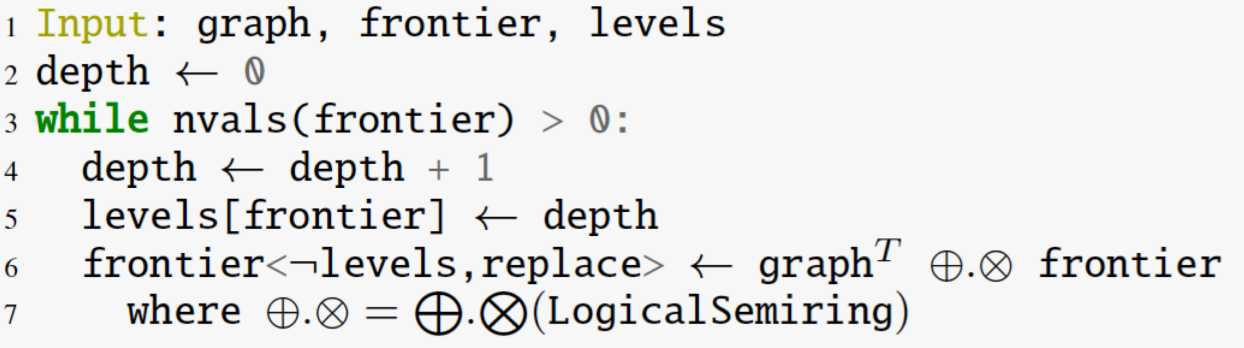
\includegraphics[scale=0.4]{figures/graphBLAS BFS pseudocode.png}\\
Our correspondong code for BFS looks like the following:
\begin{lstlisting}
def BFS(G, frontier){
    <#logical>;
    N = |G|[0];
    levels = Zero(N, 1);
    maskedGT = G^T;
    depth = 0;
    while (sum(frontier)) {
        <#arithmetic>;
        depth += 1;
        <#logical>;
        levels[rangeFromVector(frontier)] = depth;
        mask = !(frontier^T)[Zeroes(N), 0, 1, N];
        maskedGT @= mask;
        frontier = maskedGT*frontier;
    }
    <#arithmetic>;
    return levels + (One(|levels|)~(-1));
}
\end{lstlisting}
Let's look at how this code works.  (Note: the cited slides can be helpful for understanding the linear algebra aspects of the algorithm.). It takes in an $n\times n$ adjacency matrix $G$ and a column vector $frontier$ of height $n$ as well, where each entry is 0 or a true value, to denote whether that vertex is in the starting list.  On line 4, we then create $levels$, a vector of the same size as $frontier$.  This will be our output vector, as it $levels[i]$ will contain the closest distance from vertex $i$ to a vertex in frontiers, or $-1$ if its unreachable.   You'll notice that we initialize $levels$ with 0s as we will decrement on line 17.  We then make a new variable $maskedGT$ on line 5, which is just the transpose of $G$.  We do this because we are going to be modifying this matrix, but we don't want to change the original $G$.  We take the transpose because that's what allows for part of the algorithm, which I'll explain in a second, and we don't want to do that on every iteration. We then set a variable $depth$ to 0 on 6.  This will keep track of our iterations.

Then we start the while loop, which keeps going as long as there is one non-zero value in $frontier$; that is, we still have vertices we want to look at.  We then increment depth on line 9, switching quickly to arithmetic for this one line, as otherwise depth would never go above 1.  Using our range-from-vector function defined in the standard library, line 11 essentially sets $levels[i]$ equal to the current depth if $frontier[i]$ is non-zero.  That way, all the vertices that we're currently searching for have their distance in levels as the current iteration in our while loop.  This will be one more than the level, but we're going to decrement on line 17.   The key portion of this code is line 14, which multiplies $maskedGT$ and $frontier$.  Because of the way the adjacency matrix is constructed, this will give us a vector in the same format as $frontier$, only now with the vertices reachable from the vertices in the original $frontier$, and we will overwrite $frontier$ with this new frontier.  With all that I've explained so far, the algorithm would be give you the correct reachable nodes, but would run over paths to vertices for which we've already found a closer path, so depths would be wrong.

To account for this issue, on lines 12 and 13 we remove all the edges to the nodes in frontier, so that as we continue in BFS, we add a previously visited node.  We generate a mask by taking our frontier, transposing it, concatenating it down $N$ times, and negating it.  Here's an example:
$$frontier = \begin{bmatrix}0 \\1\\1\\0\\0\\1\end{bmatrix}$$
$$\begin{bmatrix}0&1&1&0&0&1\end{bmatrix}$$
$$\begin{bmatrix}
0&1&1&0&0&1\\
0&1&1&0&0&1\\
0&1&1&0&0&1\\
0&1&1&0&0&1\\
0&1&1&0&0&1\\
0&1&1&0&0&1
\end{bmatrix}$$
$$\begin{bmatrix}
1&0&0&1&1&0\\
1&0&0&1&1&0\\
1&0&0&1&1&0\\
1&0&0&1&1&0\\
1&0&0&1&1&0\\
1&0&0&1&1&0
\end{bmatrix}$$
In this map, all the ones denote edges not to items in frontier, and thus edges we can keep.  So, if we do element-wise multiplication between this mask matrix and our ongoing, masked, $G^T$, we will keep removing those edges and ensure we never revisit!
